\documentclass[12pt]{article}

\usepackage[margin=1in]{geometry}

% For vertical brace rcases
\usepackage{mathtools}
% For positioning figures
\usepackage{float}
% makes figure font bold
\usepackage{caption}
\captionsetup[figure]{labelfont=bf}
% For text generation
\usepackage{lipsum}
% For drawing
\usepackage{tikz}
% For manipulating coordinates
\usetikzlibrary{calc}
% For smaller or equal sign and not divide sign
\usepackage{amssymb}
% For the diagonal fraction
\usepackage{xfrac}
% For enumerating exercise parts with letters instead of numbers
\usepackage{enumitem}
% For dfrac, which forces the fraction to be in display mode (large) e
% even in math mode (small)
\usepackage{amsmath}
% For degree sign
\usepackage{gensymb}
% For "\mathbb" macro
\usepackage{amsfonts}
\newcommand{\N}{\mathbb{N}}
\newcommand{\Z}{\mathbb{Z}}
\newcommand{\Q}{\mathbb{Q}}
\newcommand{\R}{\mathbb{R}}
\newcommand{\C}{\mathbb{C}}
\newcommand{\F}{\mathbb{F}}
\newcommand{\rad}{\text{ rad}}

% overline short italic
\newcommand{\olsi}[1]{\,\overline{\!{#1}}}

\title{%
    \Huge Abstract Algebra \\
    \large by \\
    \Large Dummit and Foote \\~\\
    \huge Part 1: Group Theory \\
    \LARGE Chapter 2: Subgroups \\
    \Large Section 2: Centralizers and Noramlizers, Stabilizers and Kernels
}
\date{2023-07-14}
\author{Michael Saba}

\begin{document}
    \pagenumbering{gobble}
    \maketitle
    \newpage
    \pagenumbering{arabic}


    \section*{Exercise 1}
    Proof that for a group $G$ and $A \subseteq G$ where $A \neq \emptyset$,
    $C_G(A) = \{ g \in G \mid g^{-1}ag = a \; \forall a \in A\}$: \\
     We know that
    $C_G(A) = \{ g \in G \mid gag^{-1} = a \; \forall a \in A\ \}$.
    So for all $a$ in $C_G(A)$,
    \[gag^{-1} = a \iff ag^{-1} = g^{-1}a \iff a = g^{-1}ag\]
    So we can use $g^{-1}ag$ instead of $g^{-1}ag$
    as an alternative way of defining the centralizer of $A$ in $G$.


    \section*{Exercise 2}
    Proof that $C_G(Z(G)) = G$ for any group $G$:
    We know that the centralizer of a set in a group is the set of elements
    in the group that commute with all elements of the set.
    So by definition, we know that the centralizer of any set in a group
    is a subset of the group. So $C_G(Z(G)) \subseteq G$.
    The center of the group on the other hand, is the set of elements
    in the group that commute with all other elements in the group.
    So the centralizer of the center in $G$, $C_G(Z(G))$,
    is the set of elements that commute with the center, which
    are by the definition of the center all elements in $G$.
    So $G \subseteq C_G(Z(G))$,
    and we already know that $C_G(Z(G)) \subseteq G$,
    which must mean that $C_G(Z(G)) = G$. \\
    Proof that $N_G(Z(G)) = G$ for any group $G$: \\
    The normalizer of a set in a group is the set of all elements in
    the group that commute set wise with group.
    This means that for each member in the normalizer,
    the set produced by left multiplying elements of the set by said
    member is the same as the set produced by right multiplying them.
    This means that the centralizer is a special case of the normalizer,
    whose elements commute with the set because they commute with
    every element of that set,
    so the centralizer of a set is a subset of the normalizer of that same
    set in the group. \\
    By definition, $N_G(Z(G)) \subseteq G$,
    and we now showed that $C_G(Z(G)) \subseteq N_G(Z(G))$,
    so as $G = C_G(Z(G))$, $G \subseteq N_G(Z(G))$,
    hence $N_G(Z(G)) = G$.


    \section*{Exercise 3}
    Proof that for a group $G$, if $A, B \subseteq G$ and $A \subset B$,
    then $C_G(B) \leqslant C_G(A)$: \\
    Since $C_G(B)$ is a subgroup of $G$,
    it already fuffils all of the subgroup axioms that would make
    it a subgroup of $C_G(A)$ (closure and being non-empty)
    except for the one about being a subset of $C_G(A)$,
    which we will now prove. \\
    Since a centralizer of a set in $G$ is the set of elements in $G$
    that commute with all elements of that set,
    and since $A \subseteq B$,
    the all elements in the centralizer of $B$ must commute with every
    element in $A$, which are all in $B$.
    So $C_G(B) \subseteq C_G(A)$.
    We can thus conclude that $C_G(B) \leqslant C_G(A)$.


    \section*{Exercise 4}
    Lagrange's Theorem tells us that if $H \leqslant G$,
    then $|H| \mid |G|$.
    This helps us determine which elements make up a centralizer in
    the group because the centralizer is a subgroup,
    so once we have more elements than $\lceil \sfrac{|G|}{2} \rceil$,
    we can immediatly assume that the centralizer is all of $G$,
    since $|G|$ is the next largest divisor after $\sfrac{|G|}{2}$ 
    (if the group has even order).
    So the theorem does reduce the amount of work needed. \\
    For $S_3$: \\
    $C_{S_3}(\{ 1 \}) = S_3$ (all elements commute with 1) \\
    $C_{S_3}(\{(1\;2)\}) = \{1, (1\;2)\}$ \\
    $C_{S_3}(\{(1\;3)\}) = \{1, (1\;3)\}$ \\
    $C_{S_3}(\{(2\;3)\}) = \{1, (2\;3)\}$ \\
    $C_{S_3}(\{(1\;2\;3)\}) = \{1, (1\;2\;3), (1\;3\;2)\}$ \\
    $C_{S_3}(\{(1\;3\;2)\}) = \{1, (1\;3\;2), (1\;2\;3)\}$ \\
    For $D_8$: \\
    $C_{D_8}(\{ 1 \}) = D_8$ (all elements commute with 1) \\
    $C_{D_8}(\{ r \}) = \{1, r, r^2, r^3\}$ \\
    $C_{D_8}(\{ r^2 \}) = D_8$ \\
    $C_{D_8}(\{ r^3 \}) = \{1, r, r^2, r^3\}$ \\
    $C_{D_8}(\{ s \}) = \{1, r^2, s, sr^2\}$ \\
    $C_{D_8}(\{ sr \}) = \{1, sr, sr^3, r^2\}$ \\
    $C_{D_8}(\{ sr^2 \}) = \{1, sr^2, r^2, s\}$ \\
    $C_{D_8}(\{ sr^3 \}) = \{1, sr^3, sr, r^2\}$ \\
    For $Q_8$: \\
    $C_{Q_8}(\{ 1 \}) = Q_8$ (all elements commute with 1) \\
    $C_{Q_8}(\{ -1 \}) = Q_8$ \\
    $C_{Q_8}(\{ i \}) = \{ 1, -1, i, -i \}$ \\
    $C_{Q_8}(\{ j \}) = \{ 1, -1, j, -j \}$ \\
    $C_{Q_8}(\{ k \}) = \{ 1, -1, k, -k \}$ \\
    $C_{Q_8}(\{ -i \}) = \{ 1, -1, i, -i \}$ \\
    $C_{Q_8}(\{ -j \}) = \{ 1, -1, j, -j \}$ \\
    $C_{Q_8}(\{ -k \}) = \{ 1, -1, k, -k \}$


    \section*{Exercise 5}
    Proof that for $G$ and $A \leqslant G$,
    $C_G(A) = A$ and $N_G(A) = G$ for these groups and subgroups: \\
    \begin{enumerate}[label=\textbf{\alph*.}]
        \item     
            For $G = S_3$ and $A = \{ 1, (1\;2\;3), (3\;2\;1) \}$: \\
            We know from exercise 1.2.2.4 that 
            $C_G(\{1\}) = G$, $C_G(\{(1\;2\;3)\}) = A$,
            and $C_G(\{(3\;2\;1)\}) = A$.
            So $C_G(\{1, (1\;2\;3), (3\;2\;1)\})$ is the set of
            elements that commute with all 3,
            so its the intersection of the individual centralizers,
            $G \cap A \cap A = A$. So $C_G(A) = A$. \\
            On the other hand, we know that $C_G(A) \leqslant N_G(A)$,
            so $|N_G(A)| \geqslant |C_G(A)| = 3$.
            Since $(1\;2)(1\;2\;3)(1\;2)^{-1} = (1\;2)(1\;2\;3)(1\;2)
            = (3\;2\;1)$,
            and $(1\;2)(3\;2\;1)(1\;2)^{-1} = (1\;2)(3\;2\;1)(1\;2)
            = (1\;2\;3)$,
            and $(1\;2)1(1\;2)^{-1} = (1\;2)1(1\;2)
            = 1$,
            it means that $(1\;2) \in N_G(A)$,
            so as $|N_G(A)| \geqslant 4$,
            we can immediatly cocnlude by Lagrange's Theorem
            (as stated in exercises 1.2.2.4)
            that as $N_G(A) \leqslant S_3$, $|N_G(A)| = |S_3| = 6$,
            so $N_G(A) = S_3 = G$.
        \item
            For $G = D_8$ and $A = \{ 1, s, r^2, sr^2 \}$: \\
            Since all elements in $A$ commute with all elements in $A$
            (in this case),
            $|C_G(A)| \geqslant 4$,
            so by Lagrange's Theorem,
            since $C_G(A) \leqslant G$ where $|G| = 8$,
            $|C_G(A)| = 4$ or $|C_G(A)| = 8$.
            However, since $sr \neq rs$, $r \notin C_G(A)$,
            so $|C_G(A)| < 8$,
            which means that $|C_G(A)| = 4$,
            hence $C_G(A) = A$. \\
            We also know that $C_G(A) \leqslant N_G(A) \leqslant G$,
            so $|N_G(A)| \geqslant |C_G(A)| = 4$,
            so by Lagrange's theorem, $N_G(A) = 4$ or $N_G(A) = 8$.
            We have $r1r^{-1} = r^2$, $rsr^{-1} = sr^2$,
            $rr^2r^{-1} = r^2$, and $rsr^2r^{-1} = s$.
            So as $r \in N_G(A)$, $|N_G(A)| > 4$,
            so $|N_G(A)| = 8 = |D_8| = |G|$,
            hence $N_G(A) = G$.
        \item
            For $G = D_{10}$ and $A = \{ 1, r, r^2, r^3, r^4 \}$: \\
            Since all elements in $A$ commute with all elements in $A$
            (as they are all rotations),
            $|C_G(A)| \geqslant 5$,
            so by Lagrange's Theorem,
            since $C_G(A) \leqslant G$ where $|G| = 10$,
            $|C_G(A)| = 5$ or $|C_G(A)| = 10$.
            However, since $sr \neq rs$, $r \notin C_G(A)$,
            so $|C_G(A)| < 10$,
            which means that $|C_G(A)| = 5$,
            hence $C_G(A) = A$. \\
            We also know that $C_G(A) \leqslant N_G(A) \leqslant G$,
            so $|N_G(A)| \geqslant |C_G(A)| = 5$,
            so by Lagrange's theorem, $N_G(A) = 5$ or $N_G(A) = 10$.
            We have $s1s^{-1} = 1$, $srs^{-1} = r^4$,
            $sr^2s^{-1} = r^3$, $sr^3s^{-1} = r^2$, and $sr^4s^{-1} = r$.
            So as $s \in N_G(A)$, $|N_G(A)| > 5$,
            so $|N_G(A)| = 10 = |D_{10}| = |G|$,
            hence $N_G(A) = G$.
    \end{enumerate}


    \section*{Exercise 6 $***$}
    For $H \leqslant G$: \\
    \begin{enumerate}[label=\textbf{\alph*.}]
        \item    
            Proof that $H \leqslant N_G(H)$: \\
            Since it's already a subgroup of $G$,
            we already know that $H \neq \emptyset$
            and $H$ is closed under inverses and the group operation.
            So we will only need to show that $H \subseteq N_G(H)$. \\
            Now, in exercise 1.1.7.17,
            we proved that for a group $G$,
            the group action of $G$ on itself defined by
            $\phi: G \to G$ where $\phi(g) = hgh^{-1}$ for any
            $h \in G$ is an isomorphism,
            and therefore a bijection (called conjugation).
            Since we know that $H$ is more than just a subset,
            and is a subgroup, that means $H$ is a group in its own right.
            So we can repeat the same argument,
            and assert that $\phi: H \to H$ defined by conjugation
            is a bijection.
            So for any $h,g \in H$, $\phi(g) = hgh^{-1}$ permutes
            the set $H$,
            so $ hHh^{-1} = H$. \\
            We can also redo the proof, which claims that,
            since $H$ is a group, and closed under inverses and the group
            operation, then $\forall h, g_1, g_2 \in H$, where $g_1 \neq g_2$,
            $hg_1 \neq h_g2$, and $hg_1h^{-1} \neq hg_2h^{-1}$
            (because $H$ is a group, so $xa = b$ has one solution in $H$).
            So conjugation by a fixed element in $H$ permutes $H$.
            As this applies for any fixed $h \in H$,
            then $H \subseteq N_G(H)$.
            So $H \leqslant N_G(H)$. \\
            This isn't necessarily the case however,
            if $H$ is not a subgroup.
            When $H$ is not a subgroup, closure isn't guaranteed,
            and the proof no longer applies.
            To give a counterexamle, for $G = D_8$ and $H = \{r, s\}$,
            we have $rs$ not equal to $s$ or $r$, so
            $r$ doesn't permute $H$,
            which means $r$ isn't in $N_G(H)$, but is in $H$.
        \item
            Proof that $H \leqslant C_G(H)$ is and only if $H$ is abelian: \\
            Since it's already a subgroup of $G$,
            we already know that $H \neq \emptyset$
            and $H$ is closed under inverses and the group operation.
            So we will only need to show that $H \subseteq C_G(H)$. \\
            Since $H$ is abelian, then all elements in $H$
            commute with all elements of $H$.
            So ever elements in $H$ is in $C_G(H)$,
            which means $H \subseteq C_G(H)$,
            so $H \leqslant C_G(H)$. \\
            Conversely, if $H \leqslant C_G(H)$,
            then $H \subseteq C_G(H)$,
            so all elements in $H$ commute with all elements in $H$.
            This means that $H$ is abelian.
    \end{enumerate} 


    \section*{Exercise 7 $***$}
    Let $n \in \Z$ such that $n \geqslant 3$. \\
    \begin{enumerate}[label=\textbf{\alph*.}]
        \item    
            Proof that if $n$ is odd, $Z(D_{2n}) = \{1\}$: \\
            The center of a group is the set of elements that commute
            with all of the group.
            Now, we know that in $D_{2n}$,
            the elements take two forms $sr^i$ and $r^i$,
            where $0 \leqslant i < n$.
            And, from exercise 1.1.2.3, we know that $r^is = sr^{-i}$.
            We already know that reflections don't commute with each other,
            and that rotations commute with each other.
            So the center must be the set of rotations that commute with
            reflections.
            We know that rotations $r^i$ can only commute with
            reflection $sr^i$,
            if $r^isr^i = sr^ir^i$.
            This implies that $sr^{-i}r^i = sr^{2i}$,
            which means that $sr^{0} = sr^{2i}$,
            so $r^{0} = r^{2i}$,
            hence $r^{2i} = 0$.
            We know that $n$ is the order of $r$,
            so $n$ is the smallest value to the power which $r$
            becomes the identity (other than 0).
            We also know that the second largest number with this
            property is $2n$.
            Since $i < n$, $2i < 2n$.
            That means that $r^{2i} = 0$, $2i = n$ or $2i = 0$.
            However, we know that $2i \neq n$ since we assumed $n$ was odd.
            So $2i = 0$, which means that $r^i = 1$.
            So $1$ is the only element that commutes with relfections
            and rotations,
            meaning that $Z(D_{2n}) = \{1\}$.
        \item
            Proof that if $n$ is even such that $n = 2k$ where $k \in \Z$,
            then $Z(D_{2n}) = \{1, r^k\}$: \\
            The center of a group is the set of elements that commute
            with all of the group.
            Now, we know that in $D_{2n}$,
            the elements take two forms $sr^i$ and $r^i$,
            where $0 \leqslant i < n$.
            And, from exercise 1.1.2.3, we know that $r^is = sr^{-i}$.
            We already know that reflections don't commute with each other,
            and that rotations commute with each other.
            So the center must be the set of rotations that commute with
            reflections.
            We know that rotations $r^i$ can only commute with
            reflection $sr^i$,
            if $r^isr^i = sr^ir^i$.
            This implies that $sr^{-i}r^i = sr^{2i}$,
            which means that $sr^{0} = sr^{2i}$,
            so $r^{0} = r^{2i}$,
            hence $r^{2i} = 0$.
            We know that $n$ is the order of $r$,
            so $n$ is the smallest value to the power which $r$
            becomes the identity (other than 0).
            We also know that the second largest number with this
            property is $2n$.
            Since $i < n$, $2i < 2n$.
            That means that $r^{2i} = 0$, $2i = n$ or $2i = 0$.
            We know that $n = 2k$, so if $2i = n$, $i = k$,
            and if $2i = 0$, $i = 0$.
            So the two rotations that commute with both relfections
            and rotations are $r^k$ and $r^0 = 1$.
            So $Z(D_{2n}) = \{1, r^k\}$.
    \end{enumerate}


    \section*{Exercise 8}
    Let $G = S_n$, and let $i$ be a fixed value in $A = \{1, 2 \dots n\}$,
    and let $G_i$ be the stabilizer of $i$ in $G$.
    For the group action of $S_n$ on $A$, where $\sigma(j)$
    is the element $\sigma$ permutes $j$ to,
    $G_i = \{\sigma \in G \mid \sigma(i) = i\}$.
    Proof that $G_i \leqslant G$: \\
    First, by the definition of a group action,
    we know that $\forall i \in A, 1(i) = i$.
    So $1 \in G_i$,
    meaning $G_i \neq \emptyset$. \\
    Moreover, by definition $G_i \subseteq G$. \\
    Now, to show closure under composition,
    consider $\sigma, \pi \in G_i$.
    Since $\sigma$ and $\pi$ are elements in the stabilizer of $i$,
    $\sigma(\pi(i)) = \sigma(i) = i$,
    which means $G_i$ is closed under composition. \\
    And to show closure under inverses,
    since $\sigma \in G_i$ is a permutation
    (we could have also argued that group actions are permutations),
    it means it is a bijective map $\sigma: A \to A$.
    So $\sigma(i) = i$ implies that $\sigma^{-1}(i) = i$,
    so the two the two sided inverse of $\sigma$ under composition
    is in $G_i$,
    hence $G_i$ is closed under inverses.
    We conclude that $G_i \leqslant G$. \\
    The order of $G_i$ is the number of elements in $S_n$
    that leave $i$ in place without permuting it.
    Fixing $i$ in place means permuting every other element.
    This is the equivalent of permuting $(n-1)$ elements,
    which means that $|G_i| = |S_{n-1}| = (n-1)!$.


    \section*{Exercise 9}
    For $H \leqslant G$ and a non-empty subset of $G$, $A$,
    consider the normalizer $N_H(A) = \{ h \in H \mid hAh^{-1} = A \}$
    (the difference here is that $A$ need not be a subset of $H$).
    Proof that $N_H(A) = N_G(A) \cap H$: \\
    $N_G(A)$ contains all the elements that commute with $A$ set-wise,
    so as $H \leqslant G$, $H \subseteq G$,
    which means that all elements in $H$ that commute with $A$ set-wise
    are also in $N_G(A)$.
    So $N_H(A) \subseteq N_G(A)$.
    And by definition, $N_H(A) = H$,
    so we can conclude that $N_H(A) \subseteq N_G(A) \cap H$. \\
    Moreover, any element in $N_G(A) \cap H$ both commutes with any element
    in $A$ and is in $H$, so $N_G(A) \cap H \subseteq N_H(A)$.
    So we conclude that $N_H(A) = N_G(A) \cap H$. \\
    Proof that $N_H(A) \leqslant H$: \\
    By exercise 1.2.1.10, we know that the intersection of two
    subgroups of a group is a subgroup of that group.
    So as $H \leqslant G$ and $N_G(A) \leqslant G$,
    then $N_G(A) \cap H \leqslant G$,
    so $N_H(A) \leqslant H$.


    \section*{Exercise 10 $***$}
    Proof that for $H \leqslant G$, if $|H| = 2$, then $N_G(H) = C_G(H)$: \\
    Since $H$ is a subgroup, $1 \in H$.
    So $H = \{1, h\}$.
    We know that all elements in $G$ commute with 1,
    so if $g \in N_G(H)$, we already know that $g1g^{-1} = 1$,
    so for $gHg^{-1}$ to be equal to $H$,
    there is no option other than $ghg^{-1} = h$.
    So all $g \in N_G(H)$ fuffil the requirements of $C_G(H)$.
    So $N_G(H) \subseteq C_G(H)$.
    We already know that $C_G(H) \leqslant N_G(H)$,
    hence $C_G(H) \subseteq N_G(H)$.
    We thus conclude that $C_G(H) = N_G(H)$. \\
    Proof that if $N_G(H) = G$, then $H \leqslant Z(G)$: \\
    We've already showed that in our case, $C_G(H) = N_G(H)$,
    so if $N_G(H) = G$, $C_G(H) = G$.
    So all elements in $G$ commute with $H$,
    which means that all elements in $H$ commute with $G$,
    so $H \subseteq Z(G)$.
    Since $H \leqslant G$, it satisfies all other subgroup requirements,
    which means that $H \leqslant Z(G)$.


    \section*{Exercise 11}
    Proof that for any subset $A$ of $G$, $Z(G) \leqslant N_G(A)$: \\
    We know from exercise 1.2.2.3 that if $A, B \subseteq G$,
    and $A \subseteq B$, then $C_G(B) \subseteq C_G(A)$.
    Here, we have $Z(G) = C_G(G)$,
    and $A, G \subseteq G$,
    and $A \subseteq G$, 
    so $C_G(G) \subseteq C_G(A)$,
    hence $Z(G) \subseteq C_G(A)$
    (which makes sense since any element that commutes with all elements of
    $G$ must by default commute with all elements of $A$). 
    We aslo know that $Z(G)$ is $C_G(G)$, and all centralizers
    are subgroups of $G$.
    So $Z(G)$ satisfies all other subgroup requirements
    like closure under inverses and the group operation, 
    and being non-empty.
    So we can conclude that $Z(G) \leqslant N_G(A)$.


    \section*{Exercise 12 $***$}
    Let $R$ be the set of polynomials with 4 independent variables 
    $x_1$, $x_2$, $x_3$, and $x_4$ of the form
    \[ p(x_1, x_2, x_3, x_4) = \sum_{i = 1}^{n}
    m_i(x_1^{r_{i_1}}x_2^{r_{i_2}}x_3^{r_{i_3}}x_4^{r_{i_4}}) \]
    which is a finite sum,
    and where $m_i \in \Z$,
    and $r_{i_1}, r_{i_2}, r_{i_3}, r_{i_4} \in \N$ (including 0).
    Take for example,
    \[ p = 12x_1^5x_2^7x_4 - 18x_2^3x_3 + 11x_1^^x_2x_3^3x_4^{23} \]
    Now, for each $\sigma \in S_4$,
    for all $\sigma \in S_4$,
    consider $\sigma$ the map $\sigma: R \to R$ defined by \\
    \[\sigma \cdot p(x_1, x_2, x_3, x_4)
    = p(x_{\sigma(1)}, x_{\sigma(2)}, x_{\sigma(3)}, x_{\sigma(4)})\]
    for each term in $p$'s sum.
    \begin{enumerate}[label=\textbf{\alph*.}]
        \item    
            For the polynomial $p$, $\sigma = (1\;2\;3\;4)$,
            and $\tau = (1\;2\;3)$: \\
            $\sigma \cdot p
            = 12x_2^5x_3^7x_1 - 18x_3^3x_4 + 11x_3^^x_1x_4^3x_2^{23}$ \\
            $\tau \cdot (\sigma \cdot p) = (\tau \circ \sigma) \cdot p
            = 12x_3^5x_1^7x_2 - 18x_1^3x_4 + 11x_3^^x_1x_4^3x_2^{23}$ \\
            $\sigma \cdot (\tau \cdot p) = (\sigma \circ \tau) \cdot p
            = 12x_3^5x_4^7x_2 - 18x_4^3x_1 + 11x_3^^x_4x_1^3x_2^{23}$ \\
        \item
            Proof that the all maps $\sigma: R \to R$
            form a (left) group action by $S_4$ on $R$:
            We know that 1 doesn't permute any of the elements,
            so $1 \cdot p = p$.
            Furthermore, $\forall \tau, \sigma \in S_4$
            \[\tau \cdot (\sigma \cdot p(x_1, x_2, x_3, x_4)) \]
            \[ = \tau \cdot p(x_{\sigma(1)}, x_{\sigma(2)},
            x_{\sigma(3)}, x_{\sigma(4)}) \]
            \[= p(x_{\tau(\sigma(1))}, x_{\tau(\sigma(2))},
            x_{\tau(\sigma(3))}, x_{\tau(\sigma(4))}) \]
            \[ = p(x_{(\tau \circ \sigma) \cdot 1},
            x_{(\tau \circ \sigma) \cdot 2},
            x_{(\tau \circ \sigma) \cdot 3},
            x_{(\tau \circ \sigma) \cdot 4}) \]
            \[= (\tau \circ \sigma) \cdot p(x_1, x_2, x_3, x_4) \]
            So the action is associative as a result of composition's
            associativity in $S_4$,
            making the map a (left) group action.
        \item
            Proof that the set of permutations that stabilize
            the variable $x_4$, as in, the $G_{x_4}$,
            is a subgroup of $S_4$ isomorphism to $S_3$: \\
            The set of permutations that stablize $x_4$ 
            when acting on $R$
            is the same as the set of permutations in $S_4$
            that don't permute 4. \\
            This set is $\{1, (1\;2), (1\;3), (2\;3), (1\;2\;3), (1\;3\;2)\}$.
            The set clearly forms a subgroup,
            as it is by definition a subset of $S_4$,
            it's not empty,
            and it's closed under inverses and composition
            (if none of the permutations involve the 4th element,
            then their inverses and compositions have no reason to
            permute it in any way).
            So the set forms a subgroup of $S_4$.
            Furthermore, the elements in the subgroup
            are the same elements that are in $S_3$,
            so the subgroup is isomorphic to $S_3$.
        \item
            Proof that the stabilizer $G_p$
            where $p$ is the polynomial $(x_1 + x_2)$
            forms a subgroup of $S_4$ of order 4:
            The elements of $S_4$ whose action stabilizes the element 
            of $R$, $(x_1 + x_2)$,
            is the set of permutations that don't map 1 or 2
            to any element that isn't 1 or 2, and don't map
            any elements to 1 or 2 that isn't 1 or 2.
            That means that any permutations can be part of this set
            so long as $p$ remains $(x_1 + x_2)$ or $(x_2 + x_1)$
            (since addition is commutative).
            That set is $\{1, (1\;2), (3\;4), (1\;2)(3\;4)\}$.
            Trivially, the set is a subset of $S_4$ and is non-empty.
            Moreover, the set is closed under inverses,
            since all elements are their own inverses (since it
            only contains 2-cycles or products of disjoint 2-cycles).
            Finally, the set is closed under composition,
            because all elements multiplied by themselves give
            the identity,
            $(1\;2) \circ (3\;4) = (3\;4) \circ (1\;2) = (1\;2)(3\;4)$,
            $(1\;2) \circ (1\;2)(3\;4) = (3\;4)$,
            $(1\;2)(3\;4) \circ (1\;2) = (3\;4)(1\;2) \circ (1\;2) = (3\;4)$,
            $(1\;2)(3\;4) \circ (3\;4) = (1\;2)$,
            and
            $(3\;4) \circ (1\;2)(3\;4) = (3\;4) \circ (3\;4)(1\;2) = (1\;2)$.
            So the set forms a subgroup of $S_4$ that has order 4.
        \item
            Proof that the stabilizer $G_p$
            where $p$ is the polynomial $(x_1x_2 + x_3x_4)$
            forms a subgroup of $S_4$ isomorphic to $D_8$:
            The elements of $S_4$ whose action stabilizes the element 
            of $R$, $(x_1x_2 + x_3x_4)$,
            is the set of permutations that can map any elements
            to any other elements so long
            as the pairs 1 and 2 and 3 and 4 remain in the same pairs.
            (since addition and multiplication are commutative). \\
            So $\{1, (1\;2), (3\;4), (1\;2)(3\;4),
            (1\;3)(2\;4), (1\;4)(2\;3), (1\;3\;2\;4), (1\;4\;2\;3)\}$
            is the set forming the stabilizer.
            Trivially, the set is a subset of $S_4$ and is non-empty.
            Moreover, the set is closed under inverses,
            since all elements are their own inverses (since they
            are either 2-cycles or products of disjoint 2-cycles,
            or are the 4-cycles $(1\;3\;2\;4)$ and $(1\;4\;2\;3)$
            which are each other's inverses).
            Finally, the set is closed under composition.
            Each combination can be checked.
            So the set forms a subgroup of $S_4$ that has order 8. \\
            Now, to show that this subgroup is isomorphic to $D_8$,
            consider the map
            \[ \varphi: G_{(x_1x_2 + x_3x_4)} \to D_8 \]
            which is defined by $\varphi(1\;2) = s$
            and $\varphi(1\;3\;2\;3) = r$. \\
            One way of showing that this is an homomorphism is
            to show that a subset of the stabilizer $G_{(x_1x_2 + x_3x_4)}$
            maps to the set of generators in $D_8$ and satisfies
            all of its peresentation's relations.
            First, consider the subset of $G_{(x_1x_2 + x_3x_4)}$,
            which contains $(1\;2)$ and $(1\;3\;2\;4)$.
            We have
            \[ D_8 = \langle s, r \mid s^2 = r^4 = 1, rs = sr^{-1} \rangle \]
            We have $(1\;2)^2 = 1$ as it is a 2-cycle,
            and $(1\;3\;2\;4)^4 = 1$ as it is a 4-cycle. \\
            Furthermore, $(1\;3\;2\;4) \circ (1\;2) = (1\;4)(2\;3)$,
            and $(1\;2) \circ (1\;3\;2\;4)^{-1}
            = (1\;2) \circ (1\;4\;2\;3)
            = (1\;4)(2\;3)$.
            So the relations are satisfied,
            which makes $\varphi$ a homomorphism.
            Since $(1\;2)$ and $(1\;3\;2\;4)$ generate $G_{(x_1x_2 + x_3x_4)}$,
            the map is surjective,
            and since $|G_{(x_1x_2 + x_3x_4)}| = |D_8| = 8$,
            the map is injective.
            This makes $\varphi$ a bijection,
            and by extension, an isomorphism. \\
            We can even illustrate the argument by imagining
            the set $G_{(x_1x_2 + x_3x_4)}$ acting on a set $\{1, 2, 3, 4\}$
            that represent the vertices of a square
            with the pairs 1 and 2, and 3 and 4 on opposite ends.
            The set represents all of the rigid motions that can be applied
            to a square because, by definition,
            it contains all permutations that leave the pairs 
            1 and 2, and 3 and 4, coupled,
            which translates to leaving opposite vertices oppsoite each other,
            which is what preserves the shape of the square
            (relative positions of vertices doesn't change).

            % Figure
            \begin{figure}[H]
                \centering
                % figure is a tikz drawing
                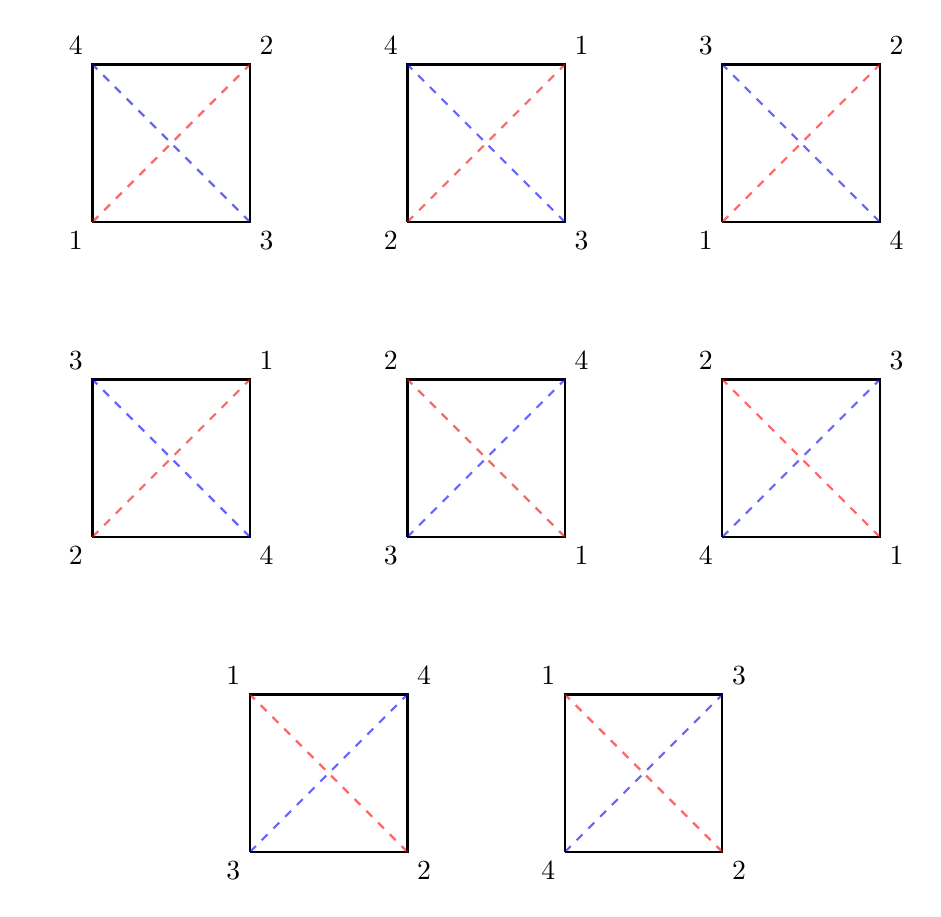
\begin{tikzpicture}[scale=2]
                % Tetrahedron formulae
                \pgfmathsetmacro{\side}{1}

                % Scope used to shift the coordinates from the basis
                \begin{scope}[shift={(0, 0, 0)}, rotate=0]
                    \coordinate (A1) at (0, 0, 0);
                    \coordinate (A2) at (\side, 0, 0);
                    \coordinate (A3) at (\side, \side, 0);                    
                    \coordinate (A4) at (0, \side, 0);

                    \coordinate (B1) at ($(A1) + (2, 0, 0)$);
                    \coordinate (B2) at ($(A2) + (2, 0, 0)$);     
                    \coordinate (B3) at ($(A3) + (2, 0, 0)$);        
                    \coordinate (B4) at ($(A4) + (2, 0, 0)$);

                    \coordinate (C1) at ($(A1) + (4, 0, 0)$);
                    \coordinate (C2) at ($(A2) + (4, 0, 0)$);     
                    \coordinate (C3) at ($(A3) + (4, 0, 0)$);        
                    \coordinate (C4) at ($(A4) + (4, 0, 0)$);

                    \coordinate (D1) at ($(A1) + (0, -2, 0)$);
                    \coordinate (D2) at ($(A2) + (0, -2, 0)$);     
                    \coordinate (D3) at ($(A3) + (0, -2, 0)$);        
                    \coordinate (D4) at ($(A4) + (0, -2, 0)$);

                    \coordinate (E1) at ($(A1) + (2, -2, 0)$);
                    \coordinate (E2) at ($(A2) + (2, -2, 0)$);     
                    \coordinate (E3) at ($(A3) + (2, -2, 0)$);        
                    \coordinate (E4) at ($(A4) + (2, -2, 0)$);

                    \coordinate (F1) at ($(A1) + (4, -2, 0)$);
                    \coordinate (F2) at ($(A2) + (4, -2, 0)$);     
                    \coordinate (F3) at ($(A3) + (4, -2, 0)$);        
                    \coordinate (F4) at ($(A4) + (4, -2, 0)$);

                    \coordinate (G1) at ($(A1) + (1, -4, 0)$);
                    \coordinate (G2) at ($(A2) + (1, -4, 0)$);     
                    \coordinate (G3) at ($(A3) + (1, -4, 0)$);        
                    \coordinate (G4) at ($(A4) + (1, -4, 0)$);

                    \coordinate (H1) at ($(A1) + (3, -4, 0)$);
                    \coordinate (H2) at ($(A2) + (3, -4, 0)$);     
                    \coordinate (H3) at ($(A3) + (3, -4, 0)$);        
                    \coordinate (H4) at ($(A4) + (3, -4, 0)$);

                    \node at (A1) [below left] {$1$};
                    \node at (A2) [below right] {$3$};
                    \node at (A3) [above right] {$2$};
                    \node at (A4) [above left] {$4$};
                    
                    \node at (B1) [below left] {$2$};
                    \node at (B2) [below right] {$3$};
                    \node at (B3) [above right] {$1$};
                    \node at (B4) [above left] {$4$};
                    
                    \node at (C1) [below left] {$1$};
                    \node at (C2) [below right] {$4$};
                    \node at (C3) [above right] {$2$};
                    \node at (C4) [above left] {$3$};
                    
                    \node at (D1) [below left] {$2$};
                    \node at (D2) [below right] {$4$};
                    \node at (D3) [above right] {$1$};
                    \node at (D4) [above left] {$3$};

                    \node at (E1) [below left] {$3$};
                    \node at (E2) [below right] {$1$};
                    \node at (E3) [above right] {$4$};
                    \node at (E4) [above left] {$2$};
                    
                    \node at (F1) [below left] {$4$};
                    \node at (F2) [below right] {$1$};
                    \node at (F3) [above right] {$3$};
                    \node at (F4) [above left] {$2$};
                    
                    \node at (G1) [below left] {$3$};
                    \node at (G2) [below right] {$2$};
                    \node at (G3) [above right] {$4$};
                    \node at (G4) [above left] {$1$};
                    
                    \node at (H1) [below left] {$4$};
                    \node at (H2) [below right] {$2$};
                    \node at (H3) [above right] {$3$};
                    \node at (H4) [above left] {$1$};
                \end{scope}

                % Draws the coordinate system basis with unit side lengths
                % Is usually transparent, remove to see it for reference
                \begin{scope}[thick, blue, line width=3, opacity=0.4,
                    transparent]
                    \draw (0, 0, 0) -- (1, 0, 0);
                    \draw (0, 0, 0) -- (0, 1, 0);
                    \draw (0, 0, 0) -- (0, 0, 1);   
                \end{scope}

                \begin{scope}[thick]
                    \draw (A1) -- (A2) -- (A3) -- (A4) -- (A1);
                    \draw (B1) -- (B2) -- (B3) -- (B4) -- (B1);
                    \draw (C1) -- (C2) -- (C3) -- (C4) -- (C1);
                    \draw (D1) -- (D2) -- (D3) -- (D4) -- (D1);
                    \draw (E1) -- (E2) -- (E3) -- (E4) -- (E1);
                    \draw (F1) -- (F2) -- (F3) -- (F4) -- (F1);
                    \draw (G1) -- (G2) -- (G3) -- (G4) -- (G1);
                    \draw (H1) -- (H2) -- (H3) -- (H4) -- (H1);
                \end{scope}

                \begin{scope}[thick,dashed,opacity=0.6]
                    \draw [red] (A1) -- (A3);
                    \draw [blue] (A2) -- (A4);

                    \draw [red] (B1) -- (B3);
                    \draw [blue] (B2) -- (B4);

                    \draw [red] (C1) -- (C3);
                    \draw [blue] (C2) -- (C4);

                    \draw [red] (D1) -- (D3);
                    \draw [blue] (D2) -- (D4);

                    \draw [blue] (E1) -- (E3);
                    \draw [red] (E2) -- (E4);

                    \draw [blue] (F1) -- (F3);
                    \draw [red] (F2) -- (F4);

                    \draw [blue] (G1) -- (G3);
                    \draw [red] (G2) -- (G4);

                    \draw [blue] (H1) -- (H3);
                    \draw [red] (H2) -- (H4);
                \end{scope}

            \end{tikzpicture}

                \caption{\label{fig:figure1} Tranformations 
                on a square that preserve relative positions.}
            \end{figure}
    
        \item
            Proof that the stabilizer $G_p$ that stabilizes
            $p = (x_1 + x_2)(x_3 + x_4)$
            are the same as those found in part e: \\
            In part e, multiplication, the operation that binds
            1 and 2, and 3 and 4 together, takes priority.
            In this part, addition now bind 1 and 2, and 3 and 4
            together, and it also takes priority,
            because paranthesis were added.
            So again, we can permute the variables however we want,
            so long as the pairs remain the same pairs. \\
            So $\{1, (1\;2), (3\;4), (1\;2)(3\;4),
            (1\;3)(2\;4), (1\;4)(2\;3), (1\;3\;2\;4), (1\;4\;2\;3)\}$
            is the set of permutations that belong in
            $G_{(x_1 + x_2)(x_3 + x_4)}$.
    \end{enumerate}


    \section*{Exercise 13}
    Suppose $R$ is the set of polynomials from exercises 1.2.2.12,
    but with $n$ independent variables instead of 4.
    For all $\sigma \in S_n$,
    consider $\sigma$ the map $\sigma: R \to R$ defined by \\
    \[\sigma \cdot p(x_1, x_2 \dots x_n)
    = p(x_{\sigma(1)}, x_{\sigma(2)} \dots x_{\sigma(n)})\]
    for each term in $p$'s sum.
    Proof that the all maps $\sigma: R \to R$
    form a (left) group action by $S_n$ on $R$:
    We know that 1 doesn't permute any of the elements,
    so $1 \cdot p = p$.
    Furthermore, $\forall \tau, \sigma \in S_n$
    \[\tau \cdot (\sigma \cdot p(x_1, x_2 \dots x_n)) \]
    \[ = \tau \cdot p(x_{\sigma(1)}, x_{\sigma(2)}, \dots x_{\sigma(n)}) \]
    \[= p(x_{\tau(\sigma(1))}, x_{\tau(\sigma(2))}
    \dots x_{\tau(\sigma(n))}) \]
    \[ = p(x_{(\tau \circ \sigma) \cdot 1},
    x_{(\tau \circ \sigma) \cdot 2}
    \dots x_{(\tau \circ \sigma) \cdot n}) \]
    \[= (\tau \circ \sigma) \cdot p(x_1, x_2 \dots x_n) \]
    So the action is associative as a result of composition's
    associativity in $S_n$,
    making the map a (left) group action.


    \section*{Exercise 14 $***$}
    For any field $F$, consider the Heisenberg group $H(F)$
    defined in exercises 1.1.4.11
    as the set
    \[\left\{ \begin{pmatrix}
        1 & a & b \\        
        0 & 1 & c \\
        0 & 0 & 1 \\
    \end{pmatrix} \; \middle\vert \; a, b, c, \in F \right\}\]
    which is a group under matrix multiplication. \\
    Now, to find the center of the Heisenberg group $Z(H(F))$,
    we need to find all matrices that commute with every matrix in $H(F)$.
    For two arbitrary matrices in $H(F)$,
    where $a, b, c, d, e, f \in F$, we have
    \[\begin{pmatrix}
        1 & a & b \\        
        0 & 1 & c \\
        0 & 0 & 1 \\
    \end{pmatrix} \cdot \begin{pmatrix}
        1 & d & e \\        
        0 & 1 & f \\
        0 & 0 & 1 \\
    \end{pmatrix}
    = \begin{pmatrix}
        1 & a + d & b + af + e \\        
        0 & 1 & c + f \\
        0 & 0 & 1 \\
    \end{pmatrix}
    \]
    and
    \[\begin{pmatrix}
        1 & d & e \\        
        0 & 1 & f \\
        0 & 0 & 1 \\
    \end{pmatrix} \cdot \begin{pmatrix}
        1 & a & b \\        
        0 & 1 & c \\
        0 & 0 & 1 \\
    \end{pmatrix}
    = \begin{pmatrix}
        1 & d + a & e + dc + b \\        
        0 & 1 & f + c \\
        0 & 0 & 1 \\
    \end{pmatrix}
    \]
    Since addition is always commutative in any field,
    $a + d = d + a$, $f + c = c + f$, and $b + e = e + b$.
    So in order for the two products to be equal,
    we only need for $af$ to be equal to $dc$. \\
    Assume with no loss of generality that the left matrix
    (the one with entries $a$, $b$, and $c$)
    is an arbitrary matrix in $H(F)$,
    and that the right matrix 
    (the one with entries $d$, $e$, and $f$)
    is a matrix in the center $Z(H(F))$.
    Since the left matrix is arbitrary, we can't regulate the values
    of $a$ and $c$ in the equation $af = dc$.
    So we must instead place the constraints on $f$ and $d$ in
    the right matrix.
    For the equation to hold for any values $a$ and $c$,
    $f$ and $d$ must be 0 (additive identity of $F$)
    since $a \cdot 0 = 0 \cdot c$ is always true. \\
    So the center $Z(H(F))$ must be the set
    \[ \left\{ \begin{pmatrix}
        1 & 0 & e \\        
        0 & 1 & 0 \\
        0 & 0 & 1 \\
    \end{pmatrix} \; \middle\vert \; e \in F \right\} \]
    Proof that $Z(H(F)) \cong F^+$: \\
    To show that the center of the Heisenberg group is isomorphic
    to the additive group of the field $F$,
    we first prove there exists a homomorphism between the two.
    Consider the map
    \[\phi: Z(H(F)) \to F^+
    \text{ defined by } \phi\left( \begin{pmatrix}
        1 & 0 & e \\        
        0 & 1 & 0 \\
        0 & 0 & 1 \\
    \end{pmatrix} \right) = e \]
    for all elements in the center. \\
    This map is clearly a homomorphism, since $\forall e, g \in F$,
    \[\begin{pmatrix}
        1 & 0 & e \\        
        0 & 1 & 0 \\
        0 & 0 & 1 \\
    \end{pmatrix} \cdot \begin{pmatrix}
        1 & 0 & g \\        
        0 & 1 & 0 \\
        0 & 0 & 1 \\
    \end{pmatrix}
    = \begin{pmatrix}
        1 & 0 & e + g \\        
        0 & 1 & 0 \\
        0 & 0 & 1 \\
    \end{pmatrix}
    \]
    and
    \[ \phi \left( \begin{pmatrix}
        1 & 0 & e \\        
        0 & 1 & 0 \\
        0 & 0 & 1 \\
    \end{pmatrix} \cdot \begin{pmatrix}
        1 & 0 & g \\        
        0 & 1 & 0 \\
        0 & 0 & 1 \\
    \end{pmatrix} \right)
    = \phi \left(\begin{pmatrix}
        1 & 0 & e + g \\        
        0 & 1 & 0 \\
        0 & 0 & 1 \\
    \end{pmatrix} \right)
    = e + g \]
    \[ = \phi \left(\begin{pmatrix}
        1 & 0 & e \\        
        0 & 1 & 0 \\
        0 & 0 & 1 \\
    \end{pmatrix} \right)
    + \phi \left(\begin{pmatrix}
        1 & 0 & g \\        
        0 & 1 & 0 \\
        0 & 0 & 1 \\
    \end{pmatrix} \right) \]
    Moreover, the mapping is trivially an injection
    because each matrix in $Z(H(F))$ is uniquely
    identified by an element in $F$,
    so the mapping to $F^+$ must also be unique,
    making $\phi$ injective
    (recall that the set $F^+$ is the same set as $F$,
    and it is $F^\times$ that is equal to $F - \{0\}$). \\
    Moreover, the mapping is surjective since 
    the center is defined as the set of matrices with an entry
    $e$ for all $e \in F$.
    So each element of the additive group $F^+$ must be the image
    of some matrix in th center $Z(H(F))$,
    making $\phi$ surjective,
    which in turns makes it a bijection. \\
    So we conclude that $\phi$ is an isomorphism,
    and $Z(H(F)) \cong F^+$.



\end{document}
